\newcommand{\NWtarget}[2]{#2}
\newcommand{\NWlink}[2]{#2}
\newcommand{\NWtxtMacroDefBy}{Fragment defined by}
\newcommand{\NWtxtMacroRefIn}{Fragment referenced in}
\newcommand{\NWtxtMacroNoRef}{Fragment never referenced}
\newcommand{\NWtxtDefBy}{Defined by}
\newcommand{\NWtxtRefIn}{Referenced in}
\newcommand{\NWtxtNoRef}{Not referenced}
\newcommand{\NWtxtFileDefBy}{File defined by}
\newcommand{\NWtxtIdentsUsed}{Uses:}
\newcommand{\NWtxtIdentsNotUsed}{Never used}
\newcommand{\NWtxtIdentsDefed}{Defines:}
\newcommand{\NWsep}{${\diamond}$}
\newcommand{\NWnotglobal}{(not defined globally)}
\newcommand{\NWuseHyperlinks}{}
\documentclass{article}
\usepackage{hyperref}
\usepackage{graphicx}
\renewcommand{\NWtarget}[2]{\hypertarget{#1}{#2}}
\renewcommand{\NWlink}[2]{\hyperlink{#1}{#2}}
\title{Slot Machine}
\author{Soham, Ke, Jagdeep}
\begin{document}
\maketitle

\section{Specification}
Users gamble with Money(Credits) which Casino provides them. Users input the bet amount and then they hit the Spin button to spin the three bars displaying the symbols.
The program comes up with a random sequence of predecided symbols.
Calculating the amount that a user wins in one spin, it adds that to total credits.
The gambling further continues until the user wants to quite or he/she runs out of coins.




\section{Analysis/Design}
Gambler will be provided with 200 credit(coins) initially, and will be given the option to adjust their bet. They can either bet 5 credits, 10 credits, 20 credits, MAX bet (50 credits). Bet amount will be deducted from their total credits as they hit the Spin button.\\

As the user hits the spin button, 3 symbols will be displayed. The sequence of symbols will thus determine the amount(credit) the user earns in that round. \\

There would be total of 10 symbols that can be used to display the sequence.\\

Determining the number of winnig credit.

\includegraphics{sequence.jpg}

A User can any time quite to walk away with the credits he/she earned or the program will be terminated as the total credit becomes less then minimum bet.\\ \\

Managing the Program:
\begin{itemize}
\item Initializing the credits to 200 and bet to 0.
\item take input from user to (via buttons) to set their bet until user hits Spin button.
\item Spin button generates a sequence of 3 symbols and display.
\item Read the sequence to determine the credits user won.
\item Change the credits accordingly.
\item Repeat until user hits the quite (withdraw) button.
\end{itemize}




\section{Implementation}
\begin{flushleft} \small
\begin{minipage}{\linewidth}\label{scrap1}\raggedright\small
\NWtarget{nuweb2a}{} \verb@"sm.cpp"@\nobreak\ {\footnotesize {2a}}$\equiv$
\vspace{-1ex}
\begin{list}{}{} \item
\mbox{}\verb@@\\
\mbox{}\verb@@\hbox{$\langle\,${\it Include files}\nobreak\ {\footnotesize \NWlink{nuweb12b}{12b}}$\,\rangle$}\verb@@\\
\mbox{}\verb@@\hbox{$\langle\,${\it Constants}\nobreak\ {\footnotesize \NWlink{nuweb13a}{13a}}$\,\rangle$}\verb@@\\
\mbox{}\verb@@\hbox{$\langle\,${\it classes}\nobreak\ {\footnotesize \NWlink{nuweb13b}{13b}}$\,\rangle$}\verb@@\\
\mbox{}\verb@@\hbox{$\langle\,${\it string fill}\nobreak\ {\footnotesize \NWlink{nuweb3}{3}}$\,\rangle$}\verb@@\\
\mbox{}\verb@@\hbox{$\langle\,${\it Select image from the data base and put the result into the box}\nobreak\ {\footnotesize \NWlink{nuweb5}{5}}$\,\rangle$}\verb@@\\
\mbox{}\verb@@\hbox{$\langle\,${\it Calculate the bet compare with spin result and give out the credits earned}\nobreak\ {\footnotesize \NWlink{nuweb6}{6}}$\,\rangle$}\verb@@\\
\mbox{}\verb@@\hbox{$\langle\,${\it Function callback}\nobreak\ {\footnotesize \NWlink{nuweb7c}{7c}}$\,\rangle$}\verb@@\\
\mbox{}\verb@@\\
\mbox{}\verb@int main()@\\
\mbox{}\verb@{@\\
\mbox{}\verb@ srand(time(0));@\\
\mbox{}\verb@@\\
\mbox{}\verb@@\hbox{$\langle\,${\it Create main window}\nobreak\ {\footnotesize \NWlink{nuweb2b}{2b}}$\,\rangle$}\verb@@\\
\mbox{}\verb@@\hbox{$\langle\,${\it Create Widgets for input and output and button}\nobreak\ {\footnotesize \NWlink{nuweb4}{4}}$\,\rangle$}\verb@@\\
\mbox{}\verb@@\hbox{$\langle\,${\it Register a callback function to be called when button is pressed}\nobreak\ {\footnotesize \NWlink{nuweb7a}{7a}}$\,\rangle$}\verb@@\\
\mbox{}\verb@@\hbox{$\langle\,${\it Show window with its controls}\nobreak\ {\footnotesize \NWlink{nuweb7b}{7b}}$\,\rangle$}\verb@@\\
\mbox{}\verb@return(Fl::run());@\\
\mbox{}\verb@ @\\
\mbox{}\verb@}@\\
\mbox{}\verb@@{\NWsep}
\end{list}
\vspace{-1.5ex}
\footnotesize
\begin{list}{}{\setlength{\itemsep}{-\parsep}\setlength{\itemindent}{-\leftmargin}}

\item{}
\end{list}
\end{minipage}\vspace{4ex}
\end{flushleft}
% Definitons of functions go here; each in their own macro
Creating main window
\begin{flushleft} \small
\begin{minipage}{\linewidth}\label{scrap2}\raggedright\small
\NWtarget{nuweb2b}{} $\langle\,${\it Create main window}\nobreak\ {\footnotesize {2b}}$\,\rangle\equiv$
\vspace{-1ex}
\begin{list}{}{} \item
\mbox{}\verb@@\\
\mbox{}\verb@Fl_Window* w = new Fl_Window(width,height);@\\
\mbox{}\verb@@{\NWsep}
\end{list}
\vspace{-1.5ex}
\footnotesize
\begin{list}{}{\setlength{\itemsep}{-\parsep}\setlength{\itemindent}{-\leftmargin}}
\item \NWtxtMacroRefIn\ \NWlink{nuweb2a}{2a}.

\item{}
\end{list}
\end{minipage}\vspace{4ex}
\end{flushleft}
This function is the generator of 3 digits that decide the sequence and display of symbols.  It Generates 3 digit unique sequence every time its called and it is used inside the spin function.
\begin{flushleft} \small
\begin{minipage}{\linewidth}\label{scrap3}\raggedright\small
\NWtarget{nuweb3}{} $\langle\,${\it string fill}\nobreak\ {\footnotesize {3}}$\,\rangle\equiv$
\vspace{-1ex}
\begin{list}{}{} \item
\mbox{}\verb@@\\
\mbox{}\verb@string fill ()@\\
\mbox{}\verb@{@\\
\mbox{}\verb@ int f;@\\
\mbox{}\verb@ ostringstream ostr;      @\\
\mbox{}\verb@ @\\
\mbox{}\verb@ f=rand()%1000;@\\
\mbox{}\verb@ ostr << setw(3) << setfill('0') << f;@\\
\mbox{}\verb@ string sequence=ostr.str();@\\
\mbox{}\verb@ @\\
\mbox{}\verb@ return sequence;@\\
\mbox{}\verb@}@\\
\mbox{}\verb@@\\
\mbox{}\verb@@{\NWsep}
\end{list}
\vspace{-1.5ex}
\footnotesize
\begin{list}{}{\setlength{\itemsep}{-\parsep}\setlength{\itemindent}{-\leftmargin}}
\item \NWtxtMacroRefIn\ \NWlink{nuweb2a}{2a}.

\item{}
\end{list}
\end{minipage}\vspace{4ex}
\end{flushleft}
Need to pass in XY coordinate (upper left corner) of box, and width, height, and label.
\begin{flushleft} \small
\begin{minipage}{\linewidth}\label{scrap4}\raggedright\small
\NWtarget{nuweb4}{} $\langle\,${\it Create Widgets for input and output and button}\nobreak\ {\footnotesize {4}}$\,\rangle\equiv$
\vspace{-1ex}
\begin{list}{}{} \item
\mbox{}\verb@@\\
\mbox{}\verb@@\\
\mbox{}\verb@@\\
\mbox{}\verb@Widgets widgets;@\\
\mbox{}\verb@widgets.credit=200;@\\
\mbox{}\verb@widgets.main_bet=0;@\\
\mbox{}\verb@@\\
\mbox{}\verb@w->begin();@\\
\mbox{}\verb@widgets.credits = new Fl_Output(100,75,150,30,"CREDITS:");@\\
\mbox{}\verb@        ostringstream ostr;          @\\
\mbox{}\verb@        ostr << widgets.credit;@\\
\mbox{}\verb@        widgets.credits->value(ostr.str().c_str());@\\
\mbox{}\verb@widgets.bet = new Fl_Output(35,350,100,25,"Bet");@\\
\mbox{}\verb@widgets.credit_earned = new Fl_Output(250,350,200,25,"Credits Earned");@\\
\mbox{}\verb@@\\
\mbox{}\verb@widgets.img[0] = new Fl_JPEG_Image("f0.jpg");@\\
\mbox{}\verb@widgets.img[1] = new Fl_JPEG_Image("f1.jpg");@\\
\mbox{}\verb@widgets.img[2] = new Fl_JPEG_Image("f2.jpg");@\\
\mbox{}\verb@widgets.img[3] = new Fl_JPEG_Image("f3.jpg");@\\
\mbox{}\verb@widgets.img[4] = new Fl_JPEG_Image("f4.jpg");@\\
\mbox{}\verb@widgets.img[5] = new Fl_JPEG_Image("f5.jpg");@\\
\mbox{}\verb@widgets.img[6] = new Fl_JPEG_Image("f6.jpg");@\\
\mbox{}\verb@widgets.img[7] = new Fl_JPEG_Image("f7.jpg");@\\
\mbox{}\verb@widgets.img[8] = new Fl_JPEG_Image("f8.jpg");@\\
\mbox{}\verb@widgets.img[9] = new Fl_JPEG_Image("f9.jpg");@\\
\mbox{}\verb@widgets.img[10] = new Fl_JPEG_Image("tfp.jpg");@\\
\mbox{}\verb@widgets.img[11] = new Fl_JPEG_Image("roc.jpg");@\\
\mbox{}\verb@@\\
\mbox{}\verb@widgets.box1 = new Fl_Box(5,125,150,200);@\\
\mbox{}\verb@widgets.box2 = new Fl_Box(158,125,150,200);@\\
\mbox{}\verb@widgets.box3 = new Fl_Box(311,125,150,200); @\\
\mbox{}\verb@@\\
\mbox{}\verb@Fl_Button* button_withdraw = new Fl_Button(480,450,160,30,"Withdraw");@\\
\mbox{}\verb@Fl_Button* button_spin = new Fl_Button(470,350,130,30,"Spin");@\\
\mbox{}\verb@Fl_Button* button_bet_again = new Fl_Button(470,300,130,30,"Bet Again");@\\
\mbox{}\verb@Fl_Button* button1 = new Fl_Button(170,400,100,30,"5 Credits");@\\
\mbox{}\verb@Fl_Button* button2 = new Fl_Button(270,400,100,30,"10 Credits");@\\
\mbox{}\verb@Fl_Button* button3 = new Fl_Button(370,400,100,30,"20 Credits");@\\
\mbox{}\verb@Fl_Button* buttonreset = new Fl_Button(50,400,100,30,"Reset");@\\
\mbox{}\verb@Fl_Button* buttonmax = new Fl_Button(490,400,100,30,"Bet Max");@\\
\mbox{}\verb@@\\
\mbox{}\verb@w->end();@\\
\mbox{}\verb@@\\
\mbox{}\verb@@{\NWsep}
\end{list}
\vspace{-1.5ex}
\footnotesize
\begin{list}{}{\setlength{\itemsep}{-\parsep}\setlength{\itemindent}{-\leftmargin}}
\item \NWtxtMacroRefIn\ \NWlink{nuweb2a}{2a}.

\item{}
\end{list}
\end{minipage}\vspace{4ex}
\end{flushleft}
This function is used to convert a string digist into integer digits and then display corresponding images. The conversion could be done by atoi function, but as these small functions were used in the framework of this program, initially, atoi failed to fit in the program.
\begin{flushleft} \small
\begin{minipage}{\linewidth}\label{scrap5}\raggedright\small
\NWtarget{nuweb5}{} $\langle\,${\it Select image from the data base and put the result into the box}\nobreak\ {\footnotesize {5}}$\,\rangle\equiv$
\vspace{-1ex}
\begin{list}{}{} \item
\mbox{}\verb@@\\
\mbox{}\verb@int select_image(char e)@\\
\mbox{}\verb@{ @\\
\mbox{}\verb@int d;@\\
\mbox{}\verb@     if (e == '0') {d=0;return d;}@\\
\mbox{}\verb@else if (e == '1') {d=1;return d;}@\\
\mbox{}\verb@else if (e == '2') {d=2;return d;}@\\
\mbox{}\verb@else if (e == '3') {d=3;return d;}@\\
\mbox{}\verb@else if (e == '4') {d=4;return d;}@\\
\mbox{}\verb@else if (e == '5') {d=5;return d;}@\\
\mbox{}\verb@else if (e == '6') {d=6;return d;}@\\
\mbox{}\verb@else if (e == '7') {d=7;return d;}@\\
\mbox{}\verb@else if (e == '8') {d=8;return d;}@\\
\mbox{}\verb@else               {d=9;return d;}@\\
\mbox{}\verb@@\\
\mbox{}\verb@}@\\
\mbox{}\verb@@\\
\mbox{}\verb@void out_image(void* v, string s)@\\
\mbox{}\verb@{@\\
\mbox{}\verb@Widgets* w = static_cast<Widgets*>(v);@\\
\mbox{}\verb@@\\
\mbox{}\verb@int a=select_image(s[0]);@\\
\mbox{}\verb@int b=select_image(s[1]);@\\
\mbox{}\verb@int c=select_image(s[2]);@\\
\mbox{}\verb@w->box1->image(w->img[a]);@\\
\mbox{}\verb@w->box1->redraw();@\\
\mbox{}\verb@w->box2->image(w->img[b]);@\\
\mbox{}\verb@w->box2->redraw();@\\
\mbox{}\verb@w->box3->image(w->img[c]);@\\
\mbox{}\verb@w->box3->redraw();@\\
\mbox{}\verb@cout << "M here in image";@\\
\mbox{}\verb@@\\
\mbox{}\verb@w->box1->parent()->redraw();@\\
\mbox{}\verb@w->box2->parent()->redraw();@\\
\mbox{}\verb@w->box3->parent()->redraw();@\\
\mbox{}\verb@@\\
\mbox{}\verb@}@\\
\mbox{}\verb@@\\
\mbox{}\verb@@{\NWsep}
\end{list}
\vspace{-1.5ex}
\footnotesize
\begin{list}{}{\setlength{\itemsep}{-\parsep}\setlength{\itemindent}{-\leftmargin}}
\item \NWtxtMacroRefIn\ \NWlink{nuweb2a}{2a}.

\item{}
\end{list}
\end{minipage}\vspace{4ex}
\end{flushleft}
This function determines the credit earned per round considerring the bet for that round.
\begin{flushleft} \small
\begin{minipage}{\linewidth}\label{scrap6}\raggedright\small
\NWtarget{nuweb6}{} $\langle\,${\it Calculate the bet compare with spin result and give out the credits earned}\nobreak\ {\footnotesize {6}}$\,\rangle\equiv$
\vspace{-1ex}
\begin{list}{}{} \item
\mbox{}\verb@@\\
\mbox{}\verb@int credit_earned(int c, int bet, string s)@\\
\mbox{}\verb@{@\\
\mbox{}\verb@char e[4];@\\
\mbox{}\verb@double p;@\\
\mbox{}\verb@strcpy(e,s.c_str());@\\
\mbox{}\verb@ @\\
\mbox{}\verb@s=s.c_str();@\\
\mbox{}\verb@@\\
\mbox{}\verb@if (bet==5){p=0.25;}@\\
\mbox{}\verb@else if (bet==10){p=0.50;}@\\
\mbox{}\verb@else if (bet==25){p=0.75;}@\\
\mbox{}\verb@else if (bet==50){p=1;}@\\
\mbox{}\verb@ @\\
\mbox{}\verb@if(s == "111") {c += p*100000000;}@\\
\mbox{}\verb@else if(s == "222") {c += p*10000000;}@\\
\mbox{}\verb@else if(s == "333") {c += p*5000000;}@\\
\mbox{}\verb@else if(s == "444") {c += p*1000000;}@\\
\mbox{}\verb@else if(s == "000") {c /= 3;}@\\
\mbox{}\verb@else if(e[0] == e[1] and e[1] == e[2]) {c += p*100000;}@\\
\mbox{}\verb@else if((e[0] == '1' and e[1] == '1') or (e[0] == '1' and e[2] == '1') or (e[2] == '1' and e[1] == '1')) {c += 100;}@\\
\mbox{}\verb@else if((e[0] == '2' and e[1] == '2') or (e[0] == '2' and e[2] == '2') or (e[2] == '2' and e[1] == '2')) {c += 80;}@\\
\mbox{}\verb@else if((e[0] == '3' and e[1] == '3') or (e[0] == '3' and e[2] == '3') or (e[2] == '3' and e[1] == '3')) {c += 75;}@\\
\mbox{}\verb@else if((e[0] == '4' and e[1] == '4') or (e[0] == '4' and e[2] == '4') or (e[2] == '4' and e[1] == '4')) {c += 50;}@\\
\mbox{}\verb@else if((e[0] == '0' and e[1] == '0') or (e[0] == '0' and e[2] == '0') or (e[2] == '0' and e[1] == '0')) {c -= bet;}@\\
\mbox{}\verb@else if(e[0] == e[2] or e[0] == e[1] or e[1] == e[2]) {c += 45;}@\\
\mbox{}\verb@else if(e[0] == '1' or e[1] == '1' or e[2] == '1') {c += 25;}@\\
\mbox{}\verb@else if(e[0] == '2' or e[1] == '2' or e[2] == '2') {c += 20;}@\\
\mbox{}\verb@else if(e[0] == '3' or e[1] == '3' or e[2] == '3') {c += 15;}@\\
\mbox{}\verb@else if(e[0] == '4' or e[1] == '4' or e[2] == '4') {c += 10;}@\\
\mbox{}\verb@else {}@\\
\mbox{}\verb@        @\\
\mbox{}\verb@ @\\
\mbox{}\verb@return c;@\\
\mbox{}\verb@}@\\
\mbox{}\verb@@\\
\mbox{}\verb@@{\NWsep}
\end{list}
\vspace{-1.5ex}
\footnotesize
\begin{list}{}{\setlength{\itemsep}{-\parsep}\setlength{\itemindent}{-\leftmargin}}
\item \NWtxtMacroRefIn\ \NWlink{nuweb2a}{2a}.

\item{}
\end{list}
\end{minipage}\vspace{4ex}
\end{flushleft}
\begin{flushleft} \small
\begin{minipage}{\linewidth}\label{scrap7}\raggedright\small
\NWtarget{nuweb7a}{} $\langle\,${\it Register a callback function to be called when button is pressed}\nobreak\ {\footnotesize {7a}}$\,\rangle\equiv$
\vspace{-1ex}
\begin{list}{}{} \item
\mbox{}\verb@@\\
\mbox{}\verb@button1->callback(bet_update_1,&widgets);@\\
\mbox{}\verb@button2->callback(bet_update_2,&widgets);@\\
\mbox{}\verb@button3->callback(bet_update_3,&widgets);@\\
\mbox{}\verb@buttonmax->callback(bet_update_max,&widgets);@\\
\mbox{}\verb@buttonreset->callback(bet_update_reset,&widgets);@\\
\mbox{}\verb@button_bet_again->callback(bet_again,&widgets);@\\
\mbox{}\verb@button_spin->callback(spin,&widgets);@\\
\mbox{}\verb@button_withdraw->callback(withdraw,&widgets);@\\
\mbox{}\verb@@{\NWsep}
\end{list}
\vspace{-1.5ex}
\footnotesize
\begin{list}{}{\setlength{\itemsep}{-\parsep}\setlength{\itemindent}{-\leftmargin}}
\item \NWtxtMacroRefIn\ \NWlink{nuweb2a}{2a}.

\item{}
\end{list}
\end{minipage}\vspace{4ex}
\end{flushleft}
\begin{flushleft} \small
\begin{minipage}{\linewidth}\label{scrap8}\raggedright\small
\NWtarget{nuweb7b}{} $\langle\,${\it Show window with its controls}\nobreak\ {\footnotesize {7b}}$\,\rangle\equiv$
\vspace{-1ex}
\begin{list}{}{} \item
\mbox{}\verb@@\\
\mbox{}\verb@w->show();@\\
\mbox{}\verb@@{\NWsep}
\end{list}
\vspace{-1.5ex}
\footnotesize
\begin{list}{}{\setlength{\itemsep}{-\parsep}\setlength{\itemindent}{-\leftmargin}}
\item \NWtxtMacroRefIn\ \NWlink{nuweb2a}{2a}.

\item{}
\end{list}
\end{minipage}\vspace{4ex}
\end{flushleft}
These are the callback functions in this program. Clicking button triggers certain codes and updates certain variables, changes displays,etc.
\begin{flushleft} \small
\begin{minipage}{\linewidth}\label{scrap9}\raggedright\small
\NWtarget{nuweb7c}{} $\langle\,${\it Function callback}\nobreak\ {\footnotesize {7c}}$\,\rangle\equiv$
\vspace{-1ex}
\begin{list}{}{} \item
\mbox{}\verb@@\\
\mbox{}\verb@@\hbox{$\langle\,${\it call back function for 5 credit bet button}\nobreak\ {\footnotesize \NWlink{nuweb8a}{8a}}$\,\rangle$}\verb@@\\
\mbox{}\verb@@\hbox{$\langle\,${\it call back function for 10 credit bet button}\nobreak\ {\footnotesize \NWlink{nuweb8b}{8b}}$\,\rangle$}\verb@@\\
\mbox{}\verb@@\hbox{$\langle\,${\it call back function for 20 credit bet button}\nobreak\ {\footnotesize \NWlink{nuweb8c}{8c}}$\,\rangle$}\verb@@\\
\mbox{}\verb@@\hbox{$\langle\,${\it call back function for max credit bet button}\nobreak\ {\footnotesize \NWlink{nuweb9a}{9a}}$\,\rangle$}\verb@@\\
\mbox{}\verb@@\hbox{$\langle\,${\it call back function for reset bet button}\nobreak\ {\footnotesize \NWlink{nuweb9b}{9b}}$\,\rangle$}\verb@@\\
\mbox{}\verb@@\hbox{$\langle\,${\it call back function for bet again button}\nobreak\ {\footnotesize \NWlink{nuweb10}{10}}$\,\rangle$}\verb@@\\
\mbox{}\verb@@\hbox{$\langle\,${\it call back function for spin button}\nobreak\ {\footnotesize \NWlink{nuweb11}{11}}$\,\rangle$}\verb@@\\
\mbox{}\verb@@\hbox{$\langle\,${\it call back function for withdraw button}\nobreak\ {\footnotesize \NWlink{nuweb12a}{12a}}$\,\rangle$}\verb@@\\
\mbox{}\verb@@{\NWsep}
\end{list}
\vspace{-1.5ex}
\footnotesize
\begin{list}{}{\setlength{\itemsep}{-\parsep}\setlength{\itemindent}{-\leftmargin}}
\item \NWtxtMacroRefIn\ \NWlink{nuweb2a}{2a}.

\item{}
\end{list}
\end{minipage}\vspace{4ex}
\end{flushleft}
call back function for 5 credit bet button. It updates the bet to 5 credits.
\begin{flushleft} \small
\begin{minipage}{\linewidth}\label{scrap10}\raggedright\small
\NWtarget{nuweb8a}{} $\langle\,${\it call back function for 5 credit bet button}\nobreak\ {\footnotesize {8a}}$\,\rangle\equiv$
\vspace{-1ex}
\begin{list}{}{} \item
\mbox{}\verb@@\\
\mbox{}\verb@void bet_update_1(Fl_Widget* o, void* v)@\\
\mbox{}\verb@{@\\
\mbox{}\verb@Widgets* w = static_cast<Widgets*>(v);@\\
\mbox{}\verb@w->main_bet=5;@\\
\mbox{}\verb@ ostringstream ostr;      @\\
\mbox{}\verb@ ostr << w->main_bet;@\\
\mbox{}\verb@ @\\
\mbox{}\verb@w->bet->value(ostr.str().c_str());@\\
\mbox{}\verb@}@\\
\mbox{}\verb@@{\NWsep}
\end{list}
\vspace{-1.5ex}
\footnotesize
\begin{list}{}{\setlength{\itemsep}{-\parsep}\setlength{\itemindent}{-\leftmargin}}
\item \NWtxtMacroRefIn\ \NWlink{nuweb7c}{7c}.

\item{}
\end{list}
\end{minipage}\vspace{4ex}
\end{flushleft}
call back function for 10 credit bet button. It updates the bet to 10 credits.
\begin{flushleft} \small
\begin{minipage}{\linewidth}\label{scrap11}\raggedright\small
\NWtarget{nuweb8b}{} $\langle\,${\it call back function for 10 credit bet button}\nobreak\ {\footnotesize {8b}}$\,\rangle\equiv$
\vspace{-1ex}
\begin{list}{}{} \item
\mbox{}\verb@@\\
\mbox{}\verb@@\\
\mbox{}\verb@void bet_update_2(Fl_Widget* o, void* v)@\\
\mbox{}\verb@{@\\
\mbox{}\verb@Widgets* w = static_cast<Widgets*>(v);@\\
\mbox{}\verb@w->main_bet=10;@\\
\mbox{}\verb@ ostringstream ostr;      @\\
\mbox{}\verb@ ostr << w->main_bet;@\\
\mbox{}\verb@@\\
\mbox{}\verb@w->bet->value(ostr.str().c_str());@\\
\mbox{}\verb@@\\
\mbox{}\verb@}@\\
\mbox{}\verb@@{\NWsep}
\end{list}
\vspace{-1.5ex}
\footnotesize
\begin{list}{}{\setlength{\itemsep}{-\parsep}\setlength{\itemindent}{-\leftmargin}}
\item \NWtxtMacroRefIn\ \NWlink{nuweb7c}{7c}.

\item{}
\end{list}
\end{minipage}\vspace{4ex}
\end{flushleft}
call back function for 20 credit bet button. It updates the bet to 20 credits.
\begin{flushleft} \small
\begin{minipage}{\linewidth}\label{scrap12}\raggedright\small
\NWtarget{nuweb8c}{} $\langle\,${\it call back function for 20 credit bet button}\nobreak\ {\footnotesize {8c}}$\,\rangle\equiv$
\vspace{-1ex}
\begin{list}{}{} \item
\mbox{}\verb@@\\
\mbox{}\verb@@\\
\mbox{}\verb@void bet_update_3(Fl_Widget* o, void* v)@\\
\mbox{}\verb@{@\\
\mbox{}\verb@Widgets* w = static_cast<Widgets*>(v);@\\
\mbox{}\verb@w->main_bet=20;@\\
\mbox{}\verb@ ostringstream ostr;      @\\
\mbox{}\verb@ ostr << w->main_bet;@\\
\mbox{}\verb@ @\\
\mbox{}\verb@w->bet->value(ostr.str().c_str());@\\
\mbox{}\verb@}@\\
\mbox{}\verb@@{\NWsep}
\end{list}
\vspace{-1.5ex}
\footnotesize
\begin{list}{}{\setlength{\itemsep}{-\parsep}\setlength{\itemindent}{-\leftmargin}}
\item \NWtxtMacroRefIn\ \NWlink{nuweb7c}{7c}.

\item{}
\end{list}
\end{minipage}\vspace{4ex}
\end{flushleft}
call back function for max credit bet button. It updates the bet to 50 credits.
\begin{flushleft} \small
\begin{minipage}{\linewidth}\label{scrap13}\raggedright\small
\NWtarget{nuweb9a}{} $\langle\,${\it call back function for max credit bet button}\nobreak\ {\footnotesize {9a}}$\,\rangle\equiv$
\vspace{-1ex}
\begin{list}{}{} \item
\mbox{}\verb@@\\
\mbox{}\verb@@\\
\mbox{}\verb@void bet_update_max(Fl_Widget* o, void* v)@\\
\mbox{}\verb@{@\\
\mbox{}\verb@Widgets* w = static_cast<Widgets*>(v);@\\
\mbox{}\verb@w->main_bet=50;@\\
\mbox{}\verb@ ostringstream ostr;      @\\
\mbox{}\verb@ ostr << w->main_bet;@\\
\mbox{}\verb@ @\\
\mbox{}\verb@w->bet->value(ostr.str().c_str());@\\
\mbox{}\verb@}@\\
\mbox{}\verb@@{\NWsep}
\end{list}
\vspace{-1.5ex}
\footnotesize
\begin{list}{}{\setlength{\itemsep}{-\parsep}\setlength{\itemindent}{-\leftmargin}}
\item \NWtxtMacroRefIn\ \NWlink{nuweb7c}{7c}.

\item{}
\end{list}
\end{minipage}\vspace{4ex}
\end{flushleft}
call back function for reseting the bet. 
\begin{flushleft} \small
\begin{minipage}{\linewidth}\label{scrap14}\raggedright\small
\NWtarget{nuweb9b}{} $\langle\,${\it call back function for reset bet button}\nobreak\ {\footnotesize {9b}}$\,\rangle\equiv$
\vspace{-1ex}
\begin{list}{}{} \item
\mbox{}\verb@@\\
\mbox{}\verb@@\\
\mbox{}\verb@@\\
\mbox{}\verb@void bet_update_reset(Fl_Widget* o, void* v)@\\
\mbox{}\verb@{@\\
\mbox{}\verb@Widgets* w = static_cast<Widgets*>(v);@\\
\mbox{}\verb@w->main_bet=0;@\\
\mbox{}\verb@ ostringstream ostr;      @\\
\mbox{}\verb@ ostr << w->main_bet;@\\
\mbox{}\verb@ @\\
\mbox{}\verb@w->bet->value(ostr.str().c_str());@\\
\mbox{}\verb@}@\\
\mbox{}\verb@@\\
\mbox{}\verb@@{\NWsep}
\end{list}
\vspace{-1.5ex}
\footnotesize
\begin{list}{}{\setlength{\itemsep}{-\parsep}\setlength{\itemindent}{-\leftmargin}}
\item \NWtxtMacroRefIn\ \NWlink{nuweb7c}{7c}.

\item{}
\end{list}
\end{minipage}\vspace{4ex}
\end{flushleft}
call back function for bet again button. It updates the credit earned output to blank and thus giving an idea of starting a new round. It shows spin button and hides itself.
\begin{flushleft} \small
\begin{minipage}{\linewidth}\label{scrap15}\raggedright\small
\NWtarget{nuweb10}{} $\langle\,${\it call back function for bet again button}\nobreak\ {\footnotesize {10}}$\,\rangle\equiv$
\vspace{-1ex}
\begin{list}{}{} \item
\mbox{}\verb@@\\
\mbox{}\verb@@\\
\mbox{}\verb@@\\
\mbox{}\verb@void bet_again(Fl_Widget* o, void* v)@\\
\mbox{}\verb@{@\\
\mbox{}\verb@Widgets* w = static_cast<Widgets*>(v);@\\
\mbox{}\verb@w->credit_earned->value("");@\\
\mbox{}\verb@@\\
\mbox{}\verb@o->parent()->child(7)->show();@\\
\mbox{}\verb@o->parent()->child(8)->hide();@\\
\mbox{}\verb@@\\
\mbox{}\verb@@\\
\mbox{}\verb@}@\\
\mbox{}\verb@@\\
\mbox{}\verb@@\\
\mbox{}\verb@@{\NWsep}
\end{list}
\vspace{-1.5ex}
\footnotesize
\begin{list}{}{\setlength{\itemsep}{-\parsep}\setlength{\itemindent}{-\leftmargin}}
\item \NWtxtMacroRefIn\ \NWlink{nuweb7c}{7c}.

\item{}
\end{list}
\end{minipage}\vspace{4ex}
\end{flushleft}
call back function for spin button. The main button which generates a sequence of 3 digit ( a string), displays the credit earned in that round by reading the 3 digit string and deciding the appropriate credit earned. It also generates the images corresponding to three digits. \\ At the end, it hides itself and shows bet again button, thus restricting users to hit the spin button again without reseting the credit earned and the bet.\\ This button also terminates the program to show that user ran out of credits when credits become lower than bet.
\begin{flushleft} \small
\begin{minipage}{\linewidth}\label{scrap16}\raggedright\small
\NWtarget{nuweb11}{} $\langle\,${\it call back function for spin button}\nobreak\ {\footnotesize {11}}$\,\rangle\equiv$
\vspace{-1ex}
\begin{list}{}{} \item
\mbox{}\verb@@\\
\mbox{}\verb@@\\
\mbox{}\verb@@\\
\mbox{}\verb@void spin(Fl_Widget* o, void* v)@\\
\mbox{}\verb@{@\\
\mbox{}\verb@Widgets* w = static_cast<Widgets*>(v);@\\
\mbox{}\verb@@\\
\mbox{}\verb@if(w->credit < 50)@\\
\mbox{}\verb@{@\\
\mbox{}\verb@        for(int i=0;i<14;i++)@\\
\mbox{}\verb@        {@\\
\mbox{}\verb@        o->parent()->child(i)->hide();@\\
\mbox{}\verb@        }@\\
\mbox{}\verb@        @\\
\mbox{}\verb@        o->parent()->child(4)->show();@\\
\mbox{}\verb@        w->box2->image(w->img[11]);@\\
\mbox{}\verb@        w->box2->redraw();@\\
\mbox{}\verb@}@\\
\mbox{}\verb@@\\
\mbox{}\verb@else@\\
\mbox{}\verb@{@\\
\mbox{}\verb@double difference;@\\
\mbox{}\verb@@\\
\mbox{}\verb@cout << "M here in spin";@\\
\mbox{}\verb@string sequence;@\\
\mbox{}\verb@sequence=fill();@\\
\mbox{}\verb@out_image(v,sequence);@\\
\mbox{}\verb@w->credit=w->credit-w->main_bet;@\\
\mbox{}\verb@double creditearned=w->credit;@\\
\mbox{}\verb@w->credit=credit_earned(w->credit,w->main_bet,sequence);@\\
\mbox{}\verb@difference=fabs(w->credit-creditearned);@\\
\mbox{}\verb@@\\
\mbox{}\verb@ ostringstream ostr;      @\\
\mbox{}\verb@ ostr << difference;@\\
\mbox{}\verb@ @\\
\mbox{}\verb@ ostringstream ostr1;     @\\
\mbox{}\verb@ ostr1 << w->credit;@\\
\mbox{}\verb@@\\
\mbox{}\verb@@\\
\mbox{}\verb@w->credit_earned->value(ostr.str().c_str());@\\
\mbox{}\verb@w->credits->value(ostr1.str().c_str());@\\
\mbox{}\verb@@\\
\mbox{}\verb@o->parent()->child(8)->show();@\\
\mbox{}\verb@o->parent()->child(7)->hide();@\\
\mbox{}\verb@}@\\
\mbox{}\verb@@\\
\mbox{}\verb@}@\\
\mbox{}\verb@@{\NWsep}
\end{list}
\vspace{-1.5ex}
\footnotesize
\begin{list}{}{\setlength{\itemsep}{-\parsep}\setlength{\itemindent}{-\leftmargin}}
\item \NWtxtMacroRefIn\ \NWlink{nuweb7c}{7c}.

\item{}
\end{list}
\end{minipage}\vspace{4ex}
\end{flushleft}
call back function for withdraw button. It hides all the buttons and outputs of the window and display an image thanking the users for playing.
\begin{flushleft} \small
\begin{minipage}{\linewidth}\label{scrap17}\raggedright\small
\NWtarget{nuweb12a}{} $\langle\,${\it call back function for withdraw button}\nobreak\ {\footnotesize {12a}}$\,\rangle\equiv$
\vspace{-1ex}
\begin{list}{}{} \item
\mbox{}\verb@@\\
\mbox{}\verb@@\\
\mbox{}\verb@@\\
\mbox{}\verb@@\\
\mbox{}\verb@@\\
\mbox{}\verb@void withdraw(Fl_Widget* o, void* v)@\\
\mbox{}\verb@{@\\
\mbox{}\verb@Widgets* w = static_cast<Widgets*>(v);@\\
\mbox{}\verb@for(int i=0;i<14;i++)@\\
\mbox{}\verb@{@\\
\mbox{}\verb@o->parent()->child(i)->hide();@\\
\mbox{}\verb@}@\\
\mbox{}\verb@@\\
\mbox{}\verb@o->parent()->child(5)->show();@\\
\mbox{}\verb@w->box3->image(w->img[10]);@\\
\mbox{}\verb@w->box3->redraw();@\\
\mbox{}\verb@}@\\
\mbox{}\verb@@\\
\mbox{}\verb@@\\
\mbox{}\verb@@\\
\mbox{}\verb@@{\NWsep}
\end{list}
\vspace{-1.5ex}
\footnotesize
\begin{list}{}{\setlength{\itemsep}{-\parsep}\setlength{\itemindent}{-\leftmargin}}
\item \NWtxtMacroRefIn\ \NWlink{nuweb7c}{7c}.

\item{}
\end{list}
\end{minipage}\vspace{4ex}
\end{flushleft}
These are the include files needed for library function calls
\begin{flushleft} \small
\begin{minipage}{\linewidth}\label{scrap18}\raggedright\small
\NWtarget{nuweb12b}{} $\langle\,${\it Include files}\nobreak\ {\footnotesize {12b}}$\,\rangle\equiv$
\vspace{-1ex}
\begin{list}{}{} \item
\mbox{}\verb@@\\
\mbox{}\verb@#include <iostream>@\\
\mbox{}\verb@#include<vector>@\\
\mbox{}\verb@#include<cmath>@\\
\mbox{}\verb@#include<cstdlib>@\\
\mbox{}\verb@#include<time.h>@\\
\mbox{}\verb@#include<sstream>@\\
\mbox{}\verb@#include<iomanip>@\\
\mbox{}\verb@#include<fl/fl.h>@\\
\mbox{}\verb@#include<fl/fl_window.h>@\\
\mbox{}\verb@#include<fl/fl_button.h>@\\
\mbox{}\verb@#include<fl/fl_output.h>@\\
\mbox{}\verb@#include<fl/fl_jpeg_image.h>@\\
\mbox{}\verb@#include<fl/fl_box.h>@\\
\mbox{}\verb@using namespace std;@\\
\mbox{}\verb@@{\NWsep}
\end{list}
\vspace{-1.5ex}
\footnotesize
\begin{list}{}{\setlength{\itemsep}{-\parsep}\setlength{\itemindent}{-\leftmargin}}
\item \NWtxtMacroRefIn\ \NWlink{nuweb2a}{2a}.

\item{}
\end{list}
\end{minipage}\vspace{4ex}
\end{flushleft}
These are the values that will not change during program execution
\begin{flushleft} \small
\begin{minipage}{\linewidth}\label{scrap19}\raggedright\small
\NWtarget{nuweb13a}{} $\langle\,${\it Constants}\nobreak\ {\footnotesize {13a}}$\,\rangle\equiv$
\vspace{-1ex}
\begin{list}{}{} \item
\mbox{}\verb@@\\
\mbox{}\verb@@\\
\mbox{}\verb@const int total_symbol = 9;@\\
\mbox{}\verb@const int symbol=3;@\\
\mbox{}\verb@const int width = 640;@\\
\mbox{}\verb@const int height = 480;@\\
\mbox{}\verb@@{\NWsep}
\end{list}
\vspace{-1.5ex}
\footnotesize
\begin{list}{}{\setlength{\itemsep}{-\parsep}\setlength{\itemindent}{-\leftmargin}}
\item \NWtxtMacroRefIn\ \NWlink{nuweb2a}{2a}.

\item{}
\end{list}
\end{minipage}\vspace{4ex}
\end{flushleft}
Classes
\begin{flushleft} \small
\begin{minipage}{\linewidth}\label{scrap20}\raggedright\small
\NWtarget{nuweb13b}{} $\langle\,${\it classes}\nobreak\ {\footnotesize {13b}}$\,\rangle\equiv$
\vspace{-1ex}
\begin{list}{}{} \item
\mbox{}\verb@@\\
\mbox{}\verb@@\\
\mbox{}\verb@struct Widgets@\\
\mbox{}\verb@{@\\
\mbox{}\verb@Fl_Output* out;@\\
\mbox{}\verb@Fl_Output* credits;@\\
\mbox{}\verb@Fl_Output* credit_earned;@\\
\mbox{}\verb@Fl_Output* bet;@\\
\mbox{}\verb@Fl_Box* box1;@\\
\mbox{}\verb@Fl_Box* box2;@\\
\mbox{}\verb@Fl_Box* box3;@\\
\mbox{}\verb@Fl_JPEG_Image* img[12];@\\
\mbox{}\verb@int main_bet;@\\
\mbox{}\verb@int credit;@\\
\mbox{}\verb@};@\\
\mbox{}\verb@@\\
\mbox{}\verb@@{\NWsep}
\end{list}
\vspace{-1.5ex}
\footnotesize
\begin{list}{}{\setlength{\itemsep}{-\parsep}\setlength{\itemindent}{-\leftmargin}}
\item \NWtxtMacroRefIn\ \NWlink{nuweb2a}{2a}.

\item{}
\end{list}
\end{minipage}\vspace{4ex}
\end{flushleft}
\section{Test}
%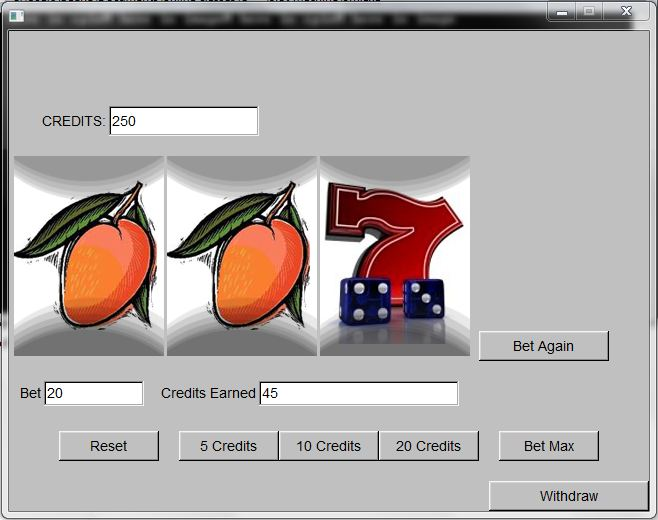
\includegraphics[scale=0.5]{lab.jpg}
\end{document}

